\section{VLANs in Proxmox}

To separate the different services and to have a more secure network, it is a good idea to use VLANs. To make Proxmox work with IEEE802.1Q VLANs, the network configuraton has to be adapted accordingly.

There are multiple possible solution to manage VLANs in Proxmox. 
\subsection{VLAN-aware Bridge and VLAN Tags}
The first and the one with the least configuration neccessary is to simply make your network bridge VLAN-aware. This can be achieved under the node-level in System $\rightarrow$ Network. 

Physical Ports can't directly be made VLAN-aware, but the corresponding bridge can be by editing the bridge and ticking the "VLAN aware" checkbox. After that, the "Apply Configuration" button has to be pressed or the changes won't be active. 
\begin{figure}[H]
	\centering
	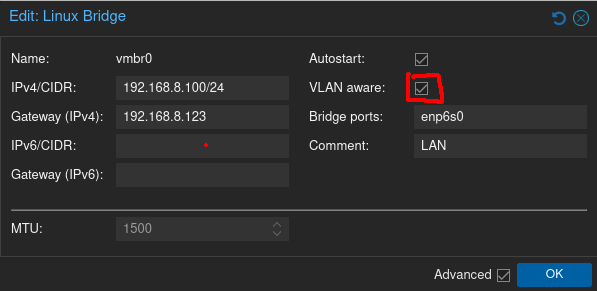
\includegraphics[width=0.8\linewidth]{Figures/vlan-aware-bridge.png}
	\caption{VLAN-aware bridge}
\end{figure}

Now to assign a VM to a VLAN, the network device of the VM has to be set to the VLAN ID. This can be done in the VM's settings under Hardware $\rightarrow$ Network Device $\rightarrow$ VLAN Tag.

\begin{figure}[H]
	\centering
	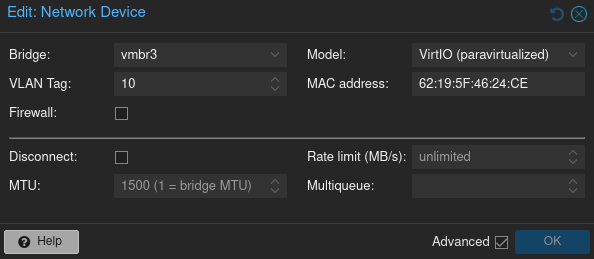
\includegraphics[width=0.8\linewidth]{Figures/vm-vlan-10.png}
	\caption{VM with VLAN ID 10}
\end{figure}

This configuration will make it possible to reach the VM from a switch connected to the bridge via a trunk link, while still encapsulating the traffic in a VLAN.

\subsection{Seperate VLAN devices}

Another solution is to create a VLAN device for each VLAN. This can be done by creating a "Linux VLAN" in the network configuration, naming it correctly using the VLAN ID and assigning it to a "raw device" which the VLAN will work on.
When using this approach, instead of assigning the VLAN ID to the VM, the VM has to be connected to the correct VLAN device.



\begin{figure}[H]
	\centering
	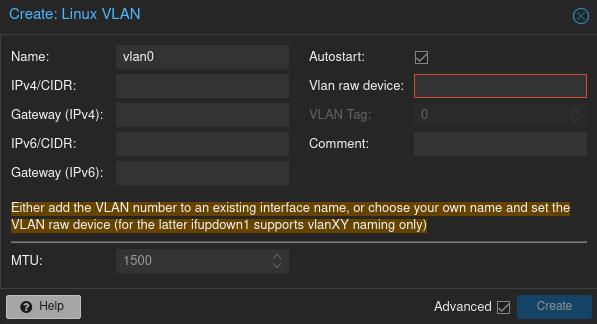
\includegraphics[width=0.8\linewidth]{Figures/linux-vlan-device.png}
	\caption{Creating a Linux VLAN device}
\end{figure}


\subsection{SDN - Software Defined Networking}
Since Proxmox VE 8.1 it is possible to use SDN to manage VLANs. This is a more complex solution, but it offers more flexibility and control over the network.
It also allows users to create Simple, QinQ, VXLAN or EVPN networks. Due to the complexity of SDN I will not go into detail here, but it is a very powerful tool to manage networks in Proxmox.

For more infos, refer to the official documentation:\\
\url{https://pve.proxmox.com/wiki/Software-Defined_Network}

\subsection{Open vSwitch VLANs}

Open vSwitch is an alternative to the Linux native bridges, bonds, and VLANs. It is a software switch that can be used as a bridge to connect VMs and containers to the network. It offers most features of a physical switch and provides some advanced features. \\
\textbf{NOTE:} Open vSwitch and Linux bridges can not be mixed! 
